% !Mode:: "TeX:UTF-8"%確保文檔utf-8編碼
\documentclass{article}

\usepackage{tikz}

\usetikzlibrary{intersections,calc,positioning,patterns,backgrounds}
% 反剪切配置
\tikzstyle{reverseclip}=[insert path={(current page.north east) --
  (current page.south east) --
  (current page.south west) --
  (current page.north west) --
  (current page.north east)}
]

\begin{document}
\begin{tikzpicture}[remember picture,overlay,scale=2]
%第一个例子
\begin{scope}[]
\begin{pgfonlayer}{background}
\fill[pattern = crosshatch] (2,0) -- (6,0) -- (6.5,0.8) --(2.5,0.8) --cycle;
\end{pgfonlayer}
\draw (0,0) -- (2,0)--(0,1)--cycle;
\draw (2.5,0.8) -- (0.5,1.8) -- (0,1);

%小车
\begin{scope}[densely dashed,xshift=0.5cm,yshift=1.2cm,rotate=-27]
\draw (-0.2,0.1) -- (0.7,0.1) --(0.7,0.3) -- (-0.2,0.3) --cycle;
\draw (-0.2,0.3) -- (0,0.5) -- (0.9,0.5) -- (0.7,0.3)--cycle;
\draw (0.7,0.1)--  (0.9,0.3) -- (0.9,0.5) -- (0.7,0.3) --cycle;
\draw (0,0) circle (0.1);
\draw (0.5,0) circle (0.1);

\begin{scope}%反剪切
\begin{pgfinterruptboundingbox}
\clip (-0.2,0.1) -- (0.7,0.1) --(0.7,0.3) -- (-0.2,0.3) --cycle [reverseclip];
\clip (-0.2,0.3) -- (0,0.5) -- (0.9,0.5) -- (0.7,0.3) --cycle [reverseclip];
\clip (0.7,0.1)--  (0.9,0.3) -- (0.9,0.5) -- (0.7,0.3)  --cycle [reverseclip];
\end{pgfinterruptboundingbox}
\draw (0.7,0.15) circle (0.1);
\draw (0.2,0.15) circle (0.1);
\end{scope}
\end{scope}
%小车复制
\begin{scope}[xshift=3cm,yshift=0.4cm,rotate=0]
\draw[fill=white] (-0.2,0.1) -- (0.7,0.1) --(0.7,0.3) -- (-0.2,0.3) --cycle;
\draw[fill=white] (-0.2,0.3) -- (0,0.5) -- (0.9,0.5) -- (0.7,0.3)--cycle;
\draw[fill=white] (0.7,0.1)--  (0.9,0.3) -- (0.9,0.5) -- (0.7,0.3) --cycle;
\draw[fill=white] (0,0) circle (0.1);
\draw[fill=white] (0.5,0) circle (0.1);

\begin{scope}%反剪切
\begin{pgfinterruptboundingbox}
\clip (-0.2,0.1) -- (0.7,0.1) --(0.7,0.3) -- (-0.2,0.3) --cycle [reverseclip];
\clip (-0.2,0.3) -- (0,0.5) -- (0.9,0.5) -- (0.7,0.3) --cycle [reverseclip];
\clip (0.7,0.1)--  (0.9,0.3) -- (0.9,0.5) -- (0.7,0.3)  --cycle [reverseclip];
\end{pgfinterruptboundingbox}
\draw[fill=white] (0.7,0.15) circle (0.1);
\draw[fill=white] (0.2,0.15) circle (0.1);
\end{scope}
\end{scope}
\end{scope}


%第二个例子
\begin{scope}[yshift=-2cm]
\begin{pgfonlayer}{background}
\fill[pattern = grid] (2,0) -- (6,0) -- (6.5,0.8) --(2.5,0.8) --cycle;
\end{pgfonlayer}
\draw (0,0) -- (2,0)--(0,1)--cycle;
\draw (2.5,0.8) -- (0.5,1.8) -- (0,1);

%小车
\begin{scope}[densely dashed,xshift=0.5cm,yshift=1.2cm,rotate=-27]
\draw (-0.2,0.1) -- (0.7,0.1) --(0.7,0.3) -- (-0.2,0.3) --cycle;
\draw (-0.2,0.3) -- (0,0.5) -- (0.9,0.5) -- (0.7,0.3)--cycle;
\draw (0.7,0.1)--  (0.9,0.3) -- (0.9,0.5) -- (0.7,0.3) --cycle;
\draw (0,0) circle (0.1);
\draw (0.5,0) circle (0.1);

\begin{scope}%反剪切
\begin{pgfinterruptboundingbox}
\clip (-0.2,0.1) -- (0.7,0.1) --(0.7,0.3) -- (-0.2,0.3) --cycle [reverseclip];
\clip (-0.2,0.3) -- (0,0.5) -- (0.9,0.5) -- (0.7,0.3) --cycle [reverseclip];
\clip (0.7,0.1)--  (0.9,0.3) -- (0.9,0.5) -- (0.7,0.3)  --cycle [reverseclip];
\end{pgfinterruptboundingbox}
\draw (0.7,0.15) circle (0.1);
\draw (0.2,0.15) circle (0.1);
\end{scope}
\end{scope}
%小车复制
\begin{scope}[xshift=4cm,yshift=0.4cm,rotate=0]
\draw[fill=white] (-0.2,0.1) -- (0.7,0.1) --(0.7,0.3) -- (-0.2,0.3) --cycle;
\draw[fill=white] (-0.2,0.3) -- (0,0.5) -- (0.9,0.5) -- (0.7,0.3)--cycle;
\draw[fill=white] (0.7,0.1)--  (0.9,0.3) -- (0.9,0.5) -- (0.7,0.3) --cycle;
\draw[fill=white] (0,0) circle (0.1);
\draw[fill=white] (0.5,0) circle (0.1);

\begin{scope}%反剪切
\begin{pgfinterruptboundingbox}
\clip (-0.2,0.1) -- (0.7,0.1) --(0.7,0.3) -- (-0.2,0.3) --cycle [reverseclip];
\clip (-0.2,0.3) -- (0,0.5) -- (0.9,0.5) -- (0.7,0.3) --cycle [reverseclip];
\clip (0.7,0.1)--  (0.9,0.3) -- (0.9,0.5) -- (0.7,0.3)  --cycle [reverseclip];
\end{pgfinterruptboundingbox}
\draw[fill=white] (0.7,0.15) circle (0.1);
\draw[fill=white] (0.2,0.15) circle (0.1);
\end{scope}
\end{scope}
\end{scope}



%第三个例子
\begin{scope}[yshift=-4cm]
\begin{pgfonlayer}{background}
\fill[pattern = horizontal lines] (2,0) -- (6,0) -- (6.5,0.8) --(2.5,0.8) --cycle;
\end{pgfonlayer}
\draw (0,0) -- (2,0)--(0,1)--cycle;
\draw (2.5,0.8) -- (0.5,1.8) -- (0,1);

%小车
\begin{scope}[densely dashed,xshift=0.5cm,yshift=1.2cm,rotate=-27]
\draw (-0.2,0.1) -- (0.7,0.1) --(0.7,0.3) -- (-0.2,0.3) --cycle;
\draw (-0.2,0.3) -- (0,0.5) -- (0.9,0.5) -- (0.7,0.3)--cycle;
\draw (0.7,0.1)--  (0.9,0.3) -- (0.9,0.5) -- (0.7,0.3) --cycle;
\draw (0,0) circle (0.1);
\draw (0.5,0) circle (0.1);

\begin{scope}%反剪切
\begin{pgfinterruptboundingbox}
\clip (-0.2,0.1) -- (0.7,0.1) --(0.7,0.3) -- (-0.2,0.3) --cycle [reverseclip];
\clip (-0.2,0.3) -- (0,0.5) -- (0.9,0.5) -- (0.7,0.3) --cycle [reverseclip];
\clip (0.7,0.1)--  (0.9,0.3) -- (0.9,0.5) -- (0.7,0.3)  --cycle [reverseclip];
\end{pgfinterruptboundingbox}
\draw (0.7,0.15) circle (0.1);
\draw (0.2,0.15) circle (0.1);
\end{scope}
\end{scope}
%小车复制
\begin{scope}[xshift=5cm,yshift=0.4cm,rotate=0]
\draw[fill=white] (-0.2,0.1) -- (0.7,0.1) --(0.7,0.3) -- (-0.2,0.3) --cycle;
\draw[fill=white] (-0.2,0.3) -- (0,0.5) -- (0.9,0.5) -- (0.7,0.3)--cycle;
\draw[fill=white] (0.7,0.1)--  (0.9,0.3) -- (0.9,0.5) -- (0.7,0.3) --cycle;
\draw[fill=white] (0,0) circle (0.1);
\draw[fill=white] (0.5,0) circle (0.1);

\begin{scope}%反剪切
\begin{pgfinterruptboundingbox}
\clip (-0.2,0.1) -- (0.7,0.1) --(0.7,0.3) -- (-0.2,0.3) --cycle [reverseclip];
\clip (-0.2,0.3) -- (0,0.5) -- (0.9,0.5) -- (0.7,0.3) --cycle [reverseclip];
\clip (0.7,0.1)--  (0.9,0.3) -- (0.9,0.5) -- (0.7,0.3)  --cycle [reverseclip];
\end{pgfinterruptboundingbox}
\draw[fill=white] (0.7,0.15) circle (0.1);
\draw[fill=white] (0.2,0.15) circle (0.1);
\end{scope}
\end{scope}
\end{scope}
\end{tikzpicture}


\end{document}